% !TeX root = ../main.tex

\chapter{研究概述与技术路线}

\section{系统整体架构}

\subsection{四槽并联AWE系统结构}

研究对象为四槽并联碱性电解水（AWE）系统，其结构如图~\ref{fig:system_architecture} 所示。
系统主要由四个并联的电解槽及其功率变换单元、碱液循环和冷却回路，以及氢侧/氧侧气液分离单元组成。

% system_structure.png 系统架构图
\begin{figure}[!htp]
  \centering
  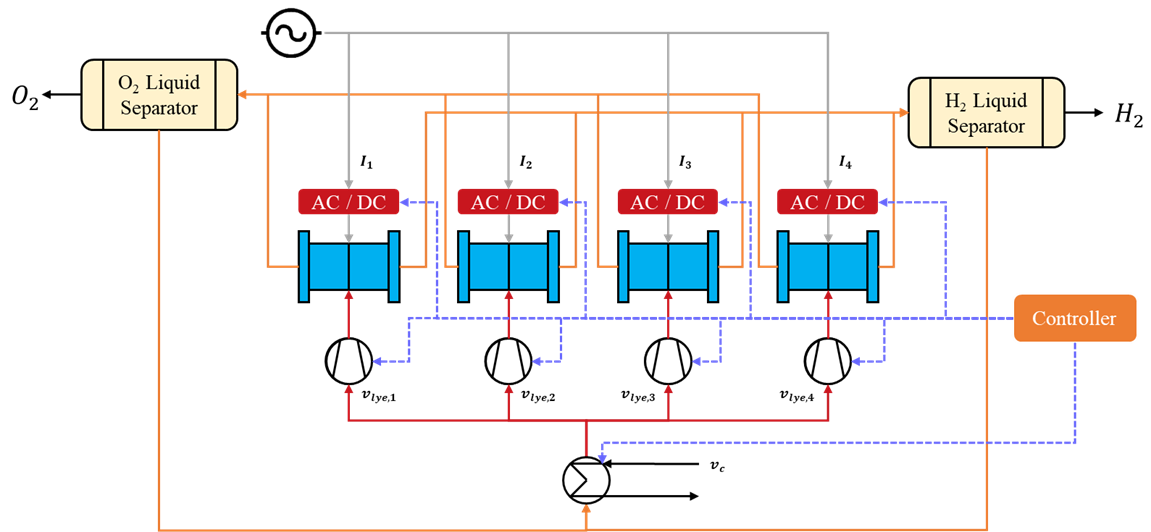
\includegraphics[width=0.95\textwidth]{figures/system_structure.png}
  \caption{四槽并联AWE系统结构示意图}
  \label{fig:system_architecture}
\end{figure}

图~\ref{fig:system_architecture} 展示了系统的三个主要功能模块：
\begin{itemize}
  \item \textbf{电-化学转换（Power \& Production）}：每个电解槽由独立的AC/DC功率变换单元调节电流，电流决定产气速率与电解槽电压，从而共同决定电功率消耗
  \item \textbf{热管理与循环回路（Heat Transfer）}：碱液循环与冷却回路共同作用，决定电解槽温度动态以及换热器的传热过程
  \item \textbf{分离与杂质传输（Separation \& Impurity）}：氢侧/氧侧气液分离与气体回路耦合，建模溶解氢、气液分配以及HTO指标演化
\end{itemize}

系统状态向量为13维：
\begin{multline}
  \mathbf{x} = [T_{s,in}, T_{s,1}, T_{s,2}, T_{s,3}, T_{s,4}, T_{sep}, T_{c,out}, \\
    n_{H_2,an,1}, n_{H_2,an,2}, n_{H_2,an,3}, n_{H_2,an,4}, n_{liq}, n_{gas}]^\top
\end{multline}

状态向量各分量含义如下：
\begin{itemize}
  \item $T_{s,in}$：换热器碱液出口温度 [K]
  \item $T_{s,i}$：第$i$个电解槽温度 [K]，$i=1,2,3,4$
  \item $T_{sep}$：分离器温度 [K]
  \item $T_{c,out}$：冷却水出口温度 [K]
  \item $n_{H_2,an,i}$：第$i$个阳极室溶解氢气摩尔数 [mol]
  \item $n_{liq}$：分离器液相氢气摩尔数 [mol]
  \item $n_{gas}$：分离器气相氢气摩尔数 [mol]
\end{itemize}

多槽系统的控制输入为9维：
\begin{equation}
  \mathbf{u} = [I_1, I_2, I_3, I_4, v_{lye,1}, v_{lye,2}, v_{lye,3}, v_{lye,4}, v_c]^\top
\end{equation}

其中$I_i$为第$i$个电解槽电流 [A]，$v_{lye,i}$为碱液流量 [$\mathrm{m}^3/\mathrm{s}$]，$v_c$为冷却水流量 [$\mathrm{m}^3/\mathrm{s}$]。

\subsection{控制目标}

系统的控制目标包括：

\begin{enumerate}
  \item \textbf{功率跟踪}：实际总功率跟踪参考功率轨迹
  \begin{equation}
    J_{track} = \sum_{k=0}^{N-1} (P_{actual,k} - P_{ref,k})^2
  \end{equation}

  \item \textbf{温度调节}：各电解槽温度维持在目标温度（通常为80°C）附近
  \begin{equation}
    J_{temp} = \sum_{k=0}^{N-1} \sum_{i=1}^{4} (T_{s,i,k} - T_{ref})^2
  \end{equation}

  \item \textbf{安全约束}：
  \begin{itemize}
    \item 温度约束：$293.15 \leq T \leq 363.15$ [K]（20--90°C）
    \item 电压约束：$U_{cell} \leq 2.2$ [V]
    \item HTO约束：$\mathrm{HTO} \leq 2$ [\%]
    \item 功率约束：$P_{stack} \leq 6$ [MW]
  \end{itemize}
\end{enumerate}

\section{技术路线对比分析}

\subsection{不同控制方法对比}

表~\ref{tab:method_comparison} 对比了所涉及的主要控制方法。

\begin{table}[!htbp]
  \centering
  \caption{不同控制方法对比}
  \label{tab:method_comparison}
  \begin{tabular}{@{}l p{3cm} p{3.5cm} p{4cm}@{}}
    \toprule
    \textbf{方法} & \textbf{核心原理} & \textbf{主要优势} & \textbf{局限性} \\
    \midrule
    NMPC & 在线非线性优化 & 理论完备，显式处理约束 & 计算开销大，实时性差 \\
    \addlinespace
    Diffusion Policy & 去噪扩散生成 & 多模态建模，高质量采样 & 推理步数多，耗时较长 \\
    \bottomrule
  \end{tabular}
\end{table}

\subsection{扩散模型的理论背景}

\textbf{1. 从行为克隆到扩散策略}

传统的模仿学习（Imitation Learning）方法，如行为克隆（Behavior Cloning），通过监督学习直接拟合专家动作：
\begin{equation}
  \pi_\theta(\mathbf{a} | \mathbf{s}) = \arg\min_\theta \mathbb{E}_{(\mathbf{s}, \mathbf{a}) \sim \mathcal{D}} [\|\mathbf{a} - \pi_\theta(\mathbf{s})\|^2]
\end{equation}

然而，行为克隆存在两个主要问题：
\begin{itemize}
  \item \textbf{分布漂移}（Distribution Shift）：训练时从专家状态分布采样，推理时从策略自身产生的状态分布采样，两者不一致导致误差累积
  \item \textbf{单峰输出}：高斯分布假设无法捕捉控制动作的多模态特性，尤其在存在多个等价最优解的场景
\end{itemize}

扩散策略（Diffusion Policy）通过建模动作的条件分布$\pi(\mathbf{a} | \mathbf{s})$而非确定性映射，有效解决了上述问题。从能量模型（Energy-based Model）的视角出发，将动作生成视为对以下分布的采样：
\begin{equation}
  p(\mathbf{a} | \mathbf{s}) \propto \exp(-E_\theta(\mathbf{a}, \mathbf{s}))
\end{equation}

其中$E_\theta$为能量函数，通过扩散过程学习。

\textbf{2. 扩散模型的控制优势}

在预测控制任务中，扩散模型相比传统方法具有以下优势：

\begin{enumerate}
  \item \textbf{多模态动作生成}：能够同时表示多个最优动作模式，而非仅输出平均值。对于功率分配问题，不同电解槽间可能存在多种等效分配方案

  \item \textbf{时间序列建模}：TCN等时序网络结构本身具有平滑性，生成的动作序列抖动较小，有利于延长执行机构寿命

  \item \textbf{可组合性}：可以与分类器引导（Classifier Guidance）或代价加权（Cost Weighting）等技术结合，实现约束满足或目标优化

  \item \textbf{模仿学习稳定性}：通过重建整个动作分布而非单点估计，对专家数据中的噪声和分布变化具有更好的容错能力
\end{enumerate}

\textbf{3. 代价加权动作选择}

生成模型输出候选动作序列后，需要通过物理仿真评估其质量，采用代价加权选择机制：
\begin{equation}
  p(\mathbf{a}^{(i)}) \propto \exp\left(-\frac{J(\mathbf{a}^{(i)})}{\alpha}\right)
\end{equation}

其中$J(\mathbf{a}^{(i)})$为第$i$个候选序列的代价，$\alpha$为温度参数。这种软选择机制平衡了探索（多样性）和利用（低代价），避免贪婪选择陷入局部最优。

\subsection{技术路线选择}

综合考虑控制性能、计算效率和实现复杂度，确定以下技术路线：

\begin{enumerate}
  \item 以NMPC作为基线方法，生成专家训练数据
  \item 重点研究Diffusion TCN策略，兼顾性能和效率
  \item 引入安全投影算子与CBF安全滤波两类安全约束保证机制，确保关键约束的严格满足
\end{enumerate}

\section{研究框架与技术路线}

\subsection{TCN Diffusion控制框架}

TCN Diffusion控制框架如图~\ref{fig:tcn_diffusion_framework} 所示。
该框架结合了时序卷积网络的长程依赖建模能力与扩散模型的高质量采样特性，
用于生成满足约束的动作序列。

\begin{figure}[!htp]
  \centering
  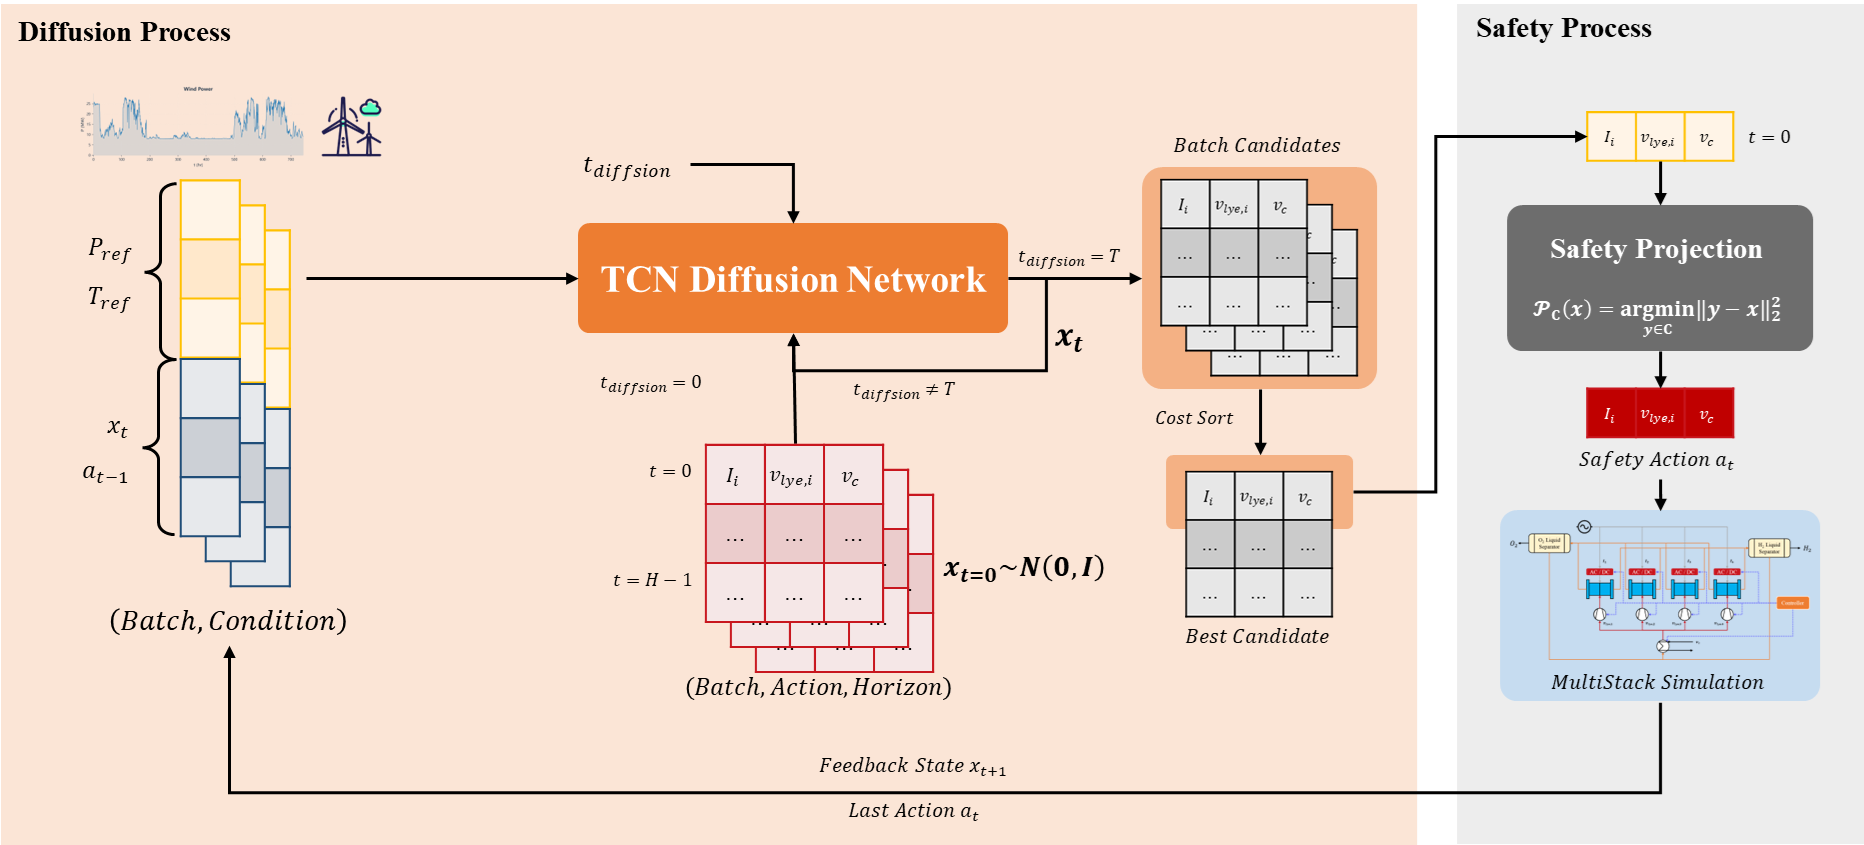
\includegraphics[width=0.98\textwidth]{figures/control_structure.png}
  \caption{TCN Diffusion控制框架图}
  \label{fig:tcn_diffusion_framework}
\end{figure}

如图~\ref{fig:tcn_diffusion_framework} 所示，该框架包含``扩散生成''和``安全约束处理''两个阶段。
TCN Diffusion网络首先从噪声中生成$K$条候选动作序列，
然后利用物理仿真对各序列进行代价评估与排序，
最终经安全投影算子或CBF安全滤波修正后执行闭环控制。

\subsection{整体研究框架}

整体研究框架如图~\ref{fig:research_framework} 所示，包括三个主要阶段：

\begin{figure}[!htp]
  \centering
  \begin{tikzpicture}[
    box/.style={rectangle, draw, rounded corners, minimum width=3cm, minimum height=1cm, align=center},
    arrow/.style={->, >=stealth, thick}
  ]
    % 阶段1
    \node[box, fill=blue!15] (phase1) at (0,0) {\textbf{阶段1：专家数据生成} \\ NMPC控制器 \\ 状态-动作轨迹};

    % 阶段2
    \node[box, fill=green!15] (phase2) at (5,0) {\textbf{阶段2：策略学习} \\ 生成模型训练 \\ Diffusion};

    % 阶段3
    \node[box, fill=orange!15] (phase3) at (10,0) {\textbf{阶段3：闭环控制} \\ 安全约束处理 \\ 实时动作选择};

    % 箭头
    \draw[arrow] (phase1) -- (phase2);
    \draw[arrow] (phase2) -- (phase3);
  \end{tikzpicture}
  \caption{研究框架示意图}
  \label{fig:research_framework}
\end{figure}

\subsection{详细技术路线}

围绕前述研究框架，技术路线可细化为以下四个阶段：

\begin{enumerate}
  \item \textbf{物理仿真建模}
  \begin{itemize}
    \item 建立电化学模型（法拉第效率、电解槽电压）
    \item 建立热力学模型（电解槽热平衡、换热器LMTD）
    \item 建立氢气传输模型（阳极室溶解、分离器分配）
    \item 实现多时间尺度ODE求解器（控制周期60s，仿真步长0.2s）
  \end{itemize}

  \item \textbf{NMPC专家数据生成}
  \begin{itemize}
    \item 设计NMPC优化问题（目标函数、约束条件）
    \item CasADi/IPOPT求解器实现
    \item Warm-starting加速策略
    \item 风电功率曲线下的大规模数据生成
  \end{itemize}

  \item \textbf{生成模型策略训练}
  \begin{itemize}
    \item 数据预处理与归一化
    \item TCN/MLP网络架构设计
    \item Diffusion训练
    \item 模型选择与超参数调优
  \end{itemize}

  \item \textbf{闭环控制与验证}
  \begin{itemize}
    \item 代价加权动作选择
    \item 投影算子安全约束保证机制
    \item 闭环仿真性能评估
    \item 与NMPC基线对比分析
  \end{itemize}
\end{enumerate}

\section{仿真平台架构}

\subsection{软件框架}

仿真平台依托Python生态构建，主要依赖包括：

\begin{itemize}
  \item \textbf{PyTorch}：神经网络训练与推理
  \item \textbf{CasADi}：NMPC优化问题建模与求解
  \item \textbf{SciPy}：ODE数值积分（solve\_ivp）
  \item \textbf{NumPy/Pandas}：数值计算与数据处理
  \item \textbf{Matplotlib}：可视化分析
\end{itemize}

\subsection{多时间尺度处理}

考虑到电解系统的动力学特性差异：

\begin{itemize}
  \item \textbf{控制周期}：$\Delta t = 60$ [s]，与实际工程实践一致
  \item \textbf{仿真步长}：$\Delta t_{sim} = 0.2$ [s]，确保数值稳定性
  \item \textbf{子步数}：每个控制周期包含$n_{sub} = 300$个仿真步
\end{itemize}

\subsection{实验数据}

采用2025年全年风电功率曲线数据作为功率参考输入：
\begin{itemize}
  \item 时间分辨率：1分钟
  \item 数据格式：CSV文件
  \item 数据范围：全年12个月，覆盖不同季节特性
\end{itemize}
